\documentclass[12pt]{article}

\usepackage{float}
\usepackage{placeins}
\usepackage{amsmath}
\usepackage{color}
\usepackage{amssymb}
\usepackage{mathtools}
\usepackage{subfigure}
\usepackage{multirow}
\usepackage{epsfig}
\usepackage{listings}
\usepackage{enumitem}
\usepackage{graphicx}    
\usepackage{graphics}
\usepackage{epstopdf}
\usepackage{longtable}
\usepackage[pdftex]{hyperref}
\usepackage{breakurl}
\usepackage{epigraph}
\usepackage{xspace}
\usepackage{amsfonts}
\usepackage{eurosym}
\usepackage{ulem}
\usepackage{footmisc}
\usepackage{comment}
\usepackage{sectsty}
\usepackage{setspace}
\usepackage{geometry}
\usepackage{caption}
\usepackage{pdflscape}
\usepackage{array}
\usepackage[round]{natbib}
\usepackage{booktabs}
\usepackage{dcolumn}
%\usepackage[justification=centering]{caption}
%\captionsetup[table]{format=plain,labelformat=simple,labelsep=period,singlelinecheck=true}%

%\bibliographystyle{unsrtnat}
\bibliographystyle{aea}
\usepackage{enumitem}
\usepackage{tikz}
\usetikzlibrary{snakes}
\usetikzlibrary{patterns}

\normalem

\doublespacing
\newtheorem{theorem}{Theorem}
\newtheorem{corollary}[theorem]{Corollary}
\newtheorem{proposition}{Proposition}
\newenvironment{proof}[1][Proof]{\noindent\textbf{#1.} }{\ \rule{0.5em}{0.5em}}
\newcommand{\ra}[1]{\renewcommand{\arraystretch}{#1}}

\newcolumntype{d}[1]{D{.}{.}{#1}} % "decimal" column type
\renewcommand{\ast}{{}^{\textstyle *}} % for raised "asterisks"

\newtheorem{hyp}{Hypothesis}
\newtheorem{subhyp}{Hypothesis}[hyp]
\renewcommand{\thesubhyp}{\thehyp\alph{subhyp}}

\newcommand{\red}[1]{{\color{red} #1}}
\newcommand{\blue}[1]{{\color{blue} #1}}

\newcommand*{\qed}{\hfill\ensuremath{\blacksquare}}%

\newcolumntype{L}[1]{>{\raggedright\let\newline\\arraybackslash\hspace{0pt}}m{#1}}
\newcolumntype{C}[1]{>{\centering\let\newline\\arraybackslash\hspace{0pt}}m{#1}}
\newcolumntype{R}[1]{>{\raggedleft\let\newline\\arraybackslash\hspace{0pt}}m{#1}}

\geometry{left=1.0in,right=1.0in,top=1.0in,bottom=1.0in}

\epstopdfsetup{outdir=./}

\newcommand{\elabel}[1]{\label{eq:#1}}
\newcommand{\eref}[1]{Eq.~(\ref{eq:#1})}
\newcommand{\ceref}[2]{(\ref{eq:#1}#2)}
\newcommand{\Eref}[1]{Equation~(\ref{eq:#1})}
\newcommand{\erefs}[2]{Eqs.~(\ref{eq:#1}--\ref{eq:#2})}

\newcommand{\Sref}[1]{Section~\ref{sec:#1}}
\newcommand{\sref}[1]{Sec.~\ref{sec:#1}}

\newcommand{\Pref}[1]{Proposition~\ref{prop:#1}}
\newcommand{\pref}[1]{Prop.~\ref{prop:#1}}
\newcommand{\preflong}[1]{proposition~\ref{prop:#1}}

\newcommand{\clabel}[1]{\label{coro:#1}}
\newcommand{\Cref}[1]{Corollary~\ref{coro:#1}}
\newcommand{\cref}[1]{Cor.~\ref{coro:#1}}
\newcommand{\creflong}[1]{corollary~\ref{coro:#1}}

\newcommand{\etal}{{\it et~al.}\xspace}
\newcommand{\ie}{{\it i.e.}\ }
\newcommand{\eg}{{\it e.g.}\ }
\newcommand{\etc}{{\it etc.}\ }
\newcommand{\cf}{{\it c.f.}\ }
\newcommand{\ave}[1]{\left\langle#1 \right\rangle}
\newcommand{\person}[1]{{\it \sc #1}}

\newcommand{\OP}[1]{{\it OP: #1 OP}}
\newcommand{\YB}[1]{{\it YB: #1 YB}}

\newcommand{\flabel}[1]{\label{fig:#1}}
\newcommand{\fref}[1]{Fig.~\ref{fig:#1}}
\newcommand{\Fref}[1]{Figure~\ref{fig:#1}}

\newcommand{\tlabel}[1]{\label{tab:#1}}
\newcommand{\tref}[1]{Tab.~\ref{tab:#1}}
\newcommand{\Tref}[1]{Table~\ref{tab:#1}}

\newcommand{\be}{\begin{equation}}
\newcommand{\ee}{\end{equation}}
\newcommand{\bea}{\begin{eqnarray*}}
\newcommand{\eea}{\end{eqnarray*}}

\newcommand{\bi}{\begin{itemize}}
\newcommand{\ei}{\end{itemize}}

\newcommand{\Dt}{\Delta t}
\newcommand{\etau}{\tau^\text{eqm}}
\newcommand{\wtau}{\widetilde{\tau}}
\newcommand{\xN}{\ave{x}_N}
\newcommand{\Sdata}{S^{\text{data}}}
\newcommand{\Smodel}{S^{\text{model}}}

\numberwithin{equation}{section}
\DeclareMathOperator\erf{erf}
%\let\endtitlepage\relax
\begin{document}

\onehalfspacing

\begin{titlepage}
\title{The relationship between relative and absolute mobility -- theory and empirics}
\author{Yonatan Berman\footnote{Paris School of Economics, Paris, France, yonatanb@post.tau.ac.il}\, and Alexander Adamou\footnote{London Mathematical Laboratory, London, UK, a.adamou@lml.org.uk} \thanks{We wish to thank Tslil Aloni, Mikkel H\o st Gandil, Ole Peters, Yoash Shapira and Alex Teytelboym for fruitful discussions and for their feedback on the manuscript.}}
\date{Original version: June 20, 2017\,\,\,\,\,\,\,\,\,\,\,\,\,\,\,\,\,\,\,\,\,\,\,\,Last updated: \today}
%\date{Last updated: \today}
\maketitle
\begin{abstract}
\noindent~\citet{chetty2014land} proposed a new measure of absolute intergenerational income mobility: the fraction of children with greater real-terms income than their parents.~\citet{chetty2017fading} studied this empirically using United States income data. They found that this measure of absolute income mobility has decreased over the last four decades. %while traditional measures of relative income mobility have remained largely stable.
They explained this as a consequence of unequal income growth. Here we establish an analytical relationship between their absolute mobility measure and traditional measures of relative mobility. % in a model in which parent and child log-incomes follow a bivariate normal distribution.
We find that the absolute mobility measure is, ceteris paribus, inversely related to traditional relative mobility measures. Additionally, our models suggest mechanisms by which changes in the marginal distributions of parent and child incomes influence absolute mobility. Our findings also offer a way to estimate absolute intergenerational mobility based on existing data on relative intergenerational mobility and on income distributions without the need for high-quality panel data sets unavailable in many countries.
%Our results are generalisable to other joint distributions of parent and child income.
\\
\\
\noindent\textbf{Keywords:} Mobility, inequality, bivariate income distributions
\\
\noindent\textbf{JEL Codes:} E0, H0, J0, R0\\

\bigskip
\end{abstract}
\setcounter{page}{0}
\thispagestyle{empty}
%\nopagebreak
\end{titlepage}
\pagebreak \newpage
%\nopagebreak

\doublespacing

\section{Introduction} \label{sec:introduction}

The ``growing public perception that intergenerational income mobility [\ldots] is declining in the United States''~\citep[p.~141]{chetty2014united} has led scholars to seek quantifiable measures of it. Typically such measures are divided into two categories, ``which capture different normative concepts''~\citep[p.~1560]{chetty2014land}, relative and absolute: relative measures gauge children's propensity to occupy a different position in the income distribution than their parents; absolute measures gauge their propensity to have higher income than their parents in money terms. A hypothetical economy in which all children have exactly twice the real incomes of their parents would exhibit minimal relative mobility and maximal absolute mobility. Therefore, the definitions of quoted mobility measures are important.

The canonical measures in each category yield different and contradictory interpretations of ostensibly the same concept, which may mislead the unaware. In addition, ``attaching a precise normative significance to `income mobility' is difficult because of the multidimensionality of this concept.''~\citep[p.~588]{fields1999measurement}

While relative intergenerational mobility has been studied for decades~\citep{becker1979equilibrium,borjas1992ethnic,mazumder2005fortunate,aaronson2008intergenerational,lee2009trends,hauser2010intergenerational,corak2013income,chetty2014united,berman2016understanding}, investigations of absolute intergenerational mobility remain ``scarce, mainly because of the lack of large, high-quality panel data sets linking children to their parents in the United States''~\citep[p.~398]{chetty2017fading}. In a recent paper,~\citet{chetty2017fading} considered trends in absolute mobility in income in the United States since 1940. They define the rate of absolute mobility as the fraction of children earning more than their parents in real terms and at the same age. They show that the rate of absolute mobility has fallen from approximately 90\% for children born in 1940 to 50\% for children born in the 1980s (see~\fref{trend}). Based on the~\citet{PSID2017},~\citet{isaacs2007economic} found that ``$67\%$ percent of Americans had higher levels of family incomes than their own parents'' (for children born during the 1950s and 1960s), agreeing with the values reported by~\citet{chetty2017fading}.

\begin{figure}[!htb]
\centering
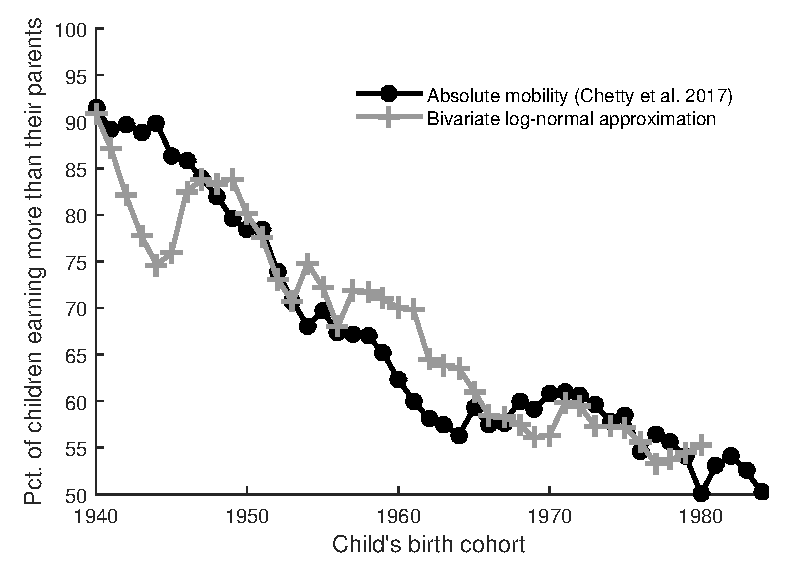
\includegraphics[width=1.0\textwidth] {./figs/trend1.eps}
\caption{A comparison between the measured (black) and approximated absolute mobility (gray). A bivariate normal distribution reproduces the historical trend of the rate of absolute mobility (the calculations are based on the pre-tax income per capita and pre-tax income distribution reported in~\citet{PikettyZucman2014} and~\citet{WID2017} assuming fixed correlation of $\rho=0.57$).}
\flabel{trend}
\end{figure}

The canonical measure of relative intergenerational mobility is the elasticity of child income with respect to parent income, known as the intergenerational earnings elasticity (IGE)~\citep{mulligan1997parental,lee2009trends,chetty2014land}. IGE is a measure of immobility rather than of mobility: the larger it is, the stronger the relationship between parent and child income. Therefore, $R_1 \equiv 1-\beta$ is used as a measure of relative mobility. Unlike absolute mobility, most empirical studies of IGE and other relative mobility measures in the United States show them holding stable over recent decades~\citep{lee2009trends,hauser2010intergenerational,chetty2014land,chetty2014united}. 

An additional important measure of relative mobility is the rank-rank slope (RRS), defined as the regression coefficient when ``regressing the child's rank on his parents' rank''~\citep[p.~1561]{chetty2014land}. Unlike the IGE, the RRS depends entirely on the copula of the joint income distribution of parents and children. The IGE also depends on the standard deviation of the log-income distributions. Therefore, it is argued that rank-rank slopes ``prove to be much more robust across specifications and are thus more suitable for comparisons across areas from a statistical perspective''~\citep[p.~1561]{chetty2014land}. Similarly to the IGE, the RRS is also a measure of immobility, and we use $R_2 \equiv 1-\text{RRS}$ as a measure of relative mobility.

Co-observations of declining absolute mobility and stable relative mobility require careful interpretation. The explanation of~\citet{chetty2017fading} for what seems to be a contrast is that income growth has been unequally distributed -- positive for high earners and stagnant for the rest -- meaning that aggregate income growth has contributed little to absolute mobility. This finding is consistent with their data but may not describe the only mechanism at work.

Here we present a theoretical study of the absolute mobility measure $A$, particularly focusing on the relationship between $A$ and the two measures of relative mobility mentioned above. We find that under a very general model of the joint log-income distribution, $A$ is inversely related to both relative mobility measures -- $R_1$ and $R_2$. We find this relationship to be robust for different copula families and marginal distributions.

Although it is argued that ``the income distribution is not well approximated by a bivariate log-normal distribution''~\citep[p.~1574]{chetty2014land}, we find that the falling absolute mobility in the US~\citep{chetty2017fading} can be well described by a bivariate normal model for the joint log-income distribution. Comparing these results to other choices of copula and marginal distribution did not improve the results.

Using the bivariate normal model, it is possible to obtain a closed-form expression for the dependencies of $A$ and $R_1$ and $A$ and $R_2$. This enables us to study mechanisms by which changes in the marginal distributions of parent and child incomes influence absolute mobility, which were not fully described in the past.

Our contribution is fourfold. Firstly, we theoretically study the relationship between distinct measures and interpretations of intergenerational mobility for the first time, suggesting that their co-movement should not, in general, be expected.

Secondly, from an empirical perspective, we are able to show that for describing the long run dynamics of absolute mobility, a model as simple as a bivariate log-normal distribution is satisfactory. This enables using powerful theoretical and empirical tools when addressing the dynamics of absolute mobility.

Thirdly, our findings suggest that using available data on the marginal income distributions and on \textit{relative} intergenerational mobility, one can produce estimates of \textit{absolute} intergenerational mobility without the need for high-quality panel data sets, which remain unavailable in most countries.

Fourthly, our study extends a body of theory of economic systems without assuming ergodicity. \YB{Alex - please complete. I am not sure of how to write this paragraph, if at all.}

\section{Model}

Our starting point is a population of $N$ parent-child pairs. We denote by $Y_p^i$ and $Y_c^i$ the incomes of the parent and the child (at the same age), respectively, in family $i=1\dots N$. We assume the incomes are all positive and define the log-incomes $X_p^i=\log Y_p^i$ and $X_c^i=\log Y_c^i$.

The intergenerational earnings elasticity (IGE) is defined as the slope ($\beta$) of the linear regression

\be
X_c = \alpha + \beta X_p + \epsilon\,,
\ee
where $\alpha$ is the regression intercept and $\epsilon$ is the error term. We define $R_1\equiv 1- \beta$ as the corresponding measure of intergenerational mobility.

The rank-rank slope (sometimes called the rank-rank correlation or Spearman's $\rho$) is defined as the correlation coefficient between the child percentile rank in the income distribution to that of parents'. We denote it by $\rho_S$ and define $R_2\equiv 1- \rho_S$ as the corresponding measure of intergenerational mobility.

The rate of absolute mobility, denoted by $A$, as defined and measured by~\citet{chetty2017fading} is the fraction of children earning more than their parents, equal to the probability $P\left(X_c-X_p > 0\right)$.

One hypothetical sample of the joint parents and children log-income distribution is presented in~\fref{lines}.~\fref{lines} also depicts how $A$ and $\beta$ are defined -- the blue line is $y=x$, hence the rate of absolute mobility is defined as the fraction of parent-child pairs which are above it. The red line is the linear regression $y=\alpha +\beta x$, for which $\beta$ is the IGE.

\begin{figure}[!htb]
\centering
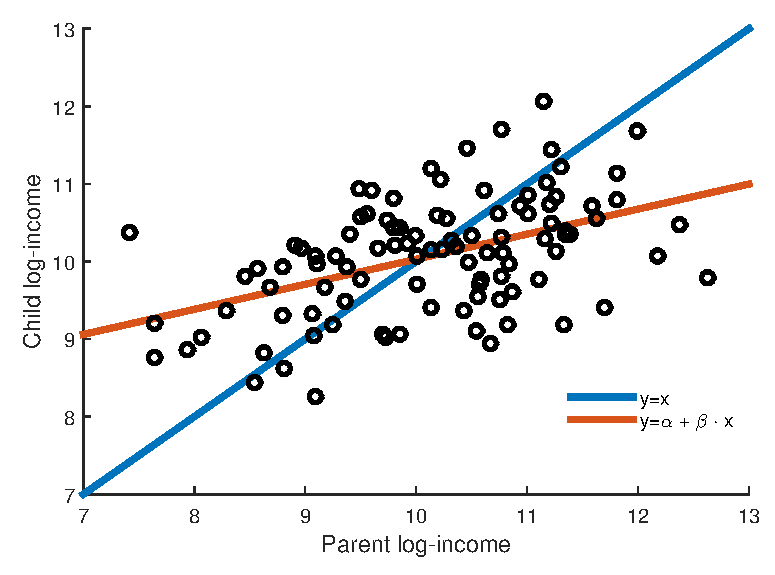
\includegraphics[width=1.0\textwidth]{./figs/bivariate_lines3.eps}
\caption{An illustration of the absolute and relative mobility measures. The black circles are a randomly chosen sample of 100 parent-child log-income pairs, assuming a bivariate normal distribution. The parameters used were $\mu_p=10.1$, $\sigma_p=0.78$ (for the parents marginal distribution) and $\mu_c=10.25$, $\sigma_c=1.15$ (for the children marginal distribution) with correlation of $\rho=0.57$. The resulting $\alpha$ and $\beta$ were $1.8$ and $0.84$, respectively.}
\flabel{lines}
\end{figure}

Since income distributions are known to be well approximated by the log-normal distribution~\citep{pinkovskiy2009parametric}, a simple plausible model for the joint distribution of parent and child log-incomes is the bivariate normal distribution. Under this assumption, the marginal income distributions of both parents and children are log-normal and the correlation between their log-incomes is defined by a single parameter $\rho$. The marginal distributions of the parents and the children follow $\mathcal{N}\left(\mu_p,\sigma_p^2\right)$ and $\mathcal{N}\left(\mu_c,\sigma_c^2\right)$, respectively. Hence the joint distribution is fully characterized by 5 parameters: $\mu_p$, $\sigma_p$, $\mu_c$, $\sigma_c$ and $\rho$.

In practice, our choice of model may affect the analysis of the absolute and relative mobility measures. Other possible models for the joint income distribution of parents and children can include marginal distributions which are not log-normal, such as beta and gamma distributions, as well as other types of copula. In the bivariate log-normal model the copula is Gaussian, while other types found useful for various empirical applications~\citep{trivedi2007copula}, such as the Clayton, the Gumbel and the Plackett copulas~\citep{bonhomme2009assessing}, may prove to be a better description of the relationship between the marginal income distributions. In their study of intergenerational mobility in France,~\citet{bonhomme2009assessing} argue that the Gaussian copula ``tends to underestimate the dependence in the middle of the distribution, that is, the probabilities of remaining in the second, third, and fourth quintiles'' and show that the empirical copula is best estimated by the Plackett copula. In Appendix~\ref{app:appB} we show that the bivariate log-normal model, with Gaussian copula, reproduces the measured historical trend of absolute mobility in the US as good as the other models tested.

\section{Results}
\label{sec:results}

We first address the properties of the bivariate log-normal approximation. In particular, we derive close form expressions for the measures of mobility -- $A$, $R_1$ and $R_2$, in terms of the distribution parameters:

\begin{proposition}
\label{prop:prop1}

For a bivariate normal distribution with parameters $\mu_p$, $\sigma_p$ (for the parents marginal distribution) and $\mu_c$, $\sigma_c$ (for the children marginal distribution) assuming correlation $\rho$, the relative mobility $R_1$ is

\be
R_1 = 1-\frac{\sigma_c}{\sigma_p}\rho \,.
\elabel{beta_rho}
\ee
\end{proposition}

Following \pref{prop1} it is also possible to derive the rate of absolute mobility as a function of the distribution parameters and the IGE:

\begin{proposition}
\label{prop:prop2}

For a bivariate normal distribution with parameters $\mu_p$, $\sigma_p$ (for the parents marginal distribution), $\mu_c$, $\sigma_c$ (for the children marginal distribution) and $\rho=\sigma_p\beta/\sigma_c$ (where $\beta$ is the IGE), the rate of absolute mobility is

\be
A = \Phi\left(\frac{\mu_c - \mu_p}{\sqrt{\sigma_p^2\left(1 - 2\beta\right) + \sigma_c^2}}\right) \,,
\elabel{abs2}
\ee
where $\Phi$ is the cumulative distribution function of the standard normal distribution.
\end{proposition}

\Eref{abs2} enables the calculation of $A$ assuming the knowledge of the marginal income distributions and $\beta$ (or $R_1$). It is therefore also possible to calculate $A$ in terms of $R_2$:

\begin{corollary}
\clabel{coro1}

Under~\pref{prop2} notations, the rate of absolute mobility $A$ is

\be
A = \Phi\left(\frac{\mu_c - \mu_p}{\sqrt{\sigma_p^2\left(1 - \frac{4\sigma_c}{\sigma_p}\sin{\left(\frac{\pi\left(1-R_2\right)}{6}\right)}\right) + \sigma_c^2}}\right) \,.
\elabel{abs3}
\ee
where $\Phi$ is the cumulative distribution function of the standard normal distribution.
\end{corollary}

Our next step is to test whether the bivariate normal model for the joint distribution of the log-incomes is empirically sound. For that purpose we compare the model prediction for the historical rate of absolute mobility in the United States with the historical rate reported by~\citet{chetty2017fading}.

We use data for the per capita pre-tax income in the United States~\citep{PikettyZucman2014} and the income share data~\citep{WID2017} to obtain $\mu_p$, $\sigma_p$, $\mu_c$ and $\sigma_c$ every year. Since in the log bivariate normal model, the marginal log-income distributions are normal, these parameters can be obtained directly and no fit is required. The Lorenz curve of the log-normal distribution $\log{\mathcal{N}}\left(\mu,\sigma^2\right)$ is $\Phi\left(\Phi^{-1}\left(z\right)-\sigma\right)$~\citep{cowell2011measuring}. Therefore, top $1\%$ income share $s$ corresponds to

\be
\sigma = \Phi^{-1}\left(0.99\right) - \Phi^{-1}\left(s\right)
\ee

If we denote the per-capita pre-tax income as $m$, it follows that the parameter $\mu$ is

\be
\mu = \log{\left(m\right)} - \frac{\sigma^2}{2}
\ee

We then use Eqs.~(\ref{eq:beta_rho}--\ref{eq:abs3}) to calculate the historical value of $A$, while fitting the correlation $\rho$ to a fixed value which minimizes the sum of squared errors from the values reported by~\citet{chetty2017fading}.

The gray curve in~\fref{trend} shows that the model reproduces faithfully the evolution of absolute mobility reported by~\citet{chetty2017fading}, despite its comparative methodological na\"{i}vety. In Appendix~\ref{app:appB} we show that this result is robsut under different choices of copula and when the gamma distribution approximation for the marginal income distributions is used instead of the log-normal approximation.

Having established the model's empirical soundness, we can use its properties to further study the measures of mobility -- $A$, $R_1$ and $R_2$. Eqs.~(\ref{eq:abs2}--\ref{eq:abs3}) demonstrate that the rate of absolute mobility can be explicitly described as a function of the relative mobility measures $R_1$ and $R_2$.~\fref{relat} shows $A$ as a function of $R_1$ and $R_2$ for different birth cohorts in the United States. It shows that the bivariate normal model -- with positive income growth and inequality changes consistent with data, but absent other effects -- predicts an \textit{inverse} relationship between absolute and relative mobility.

\begin{figure}[!htb]
\centering
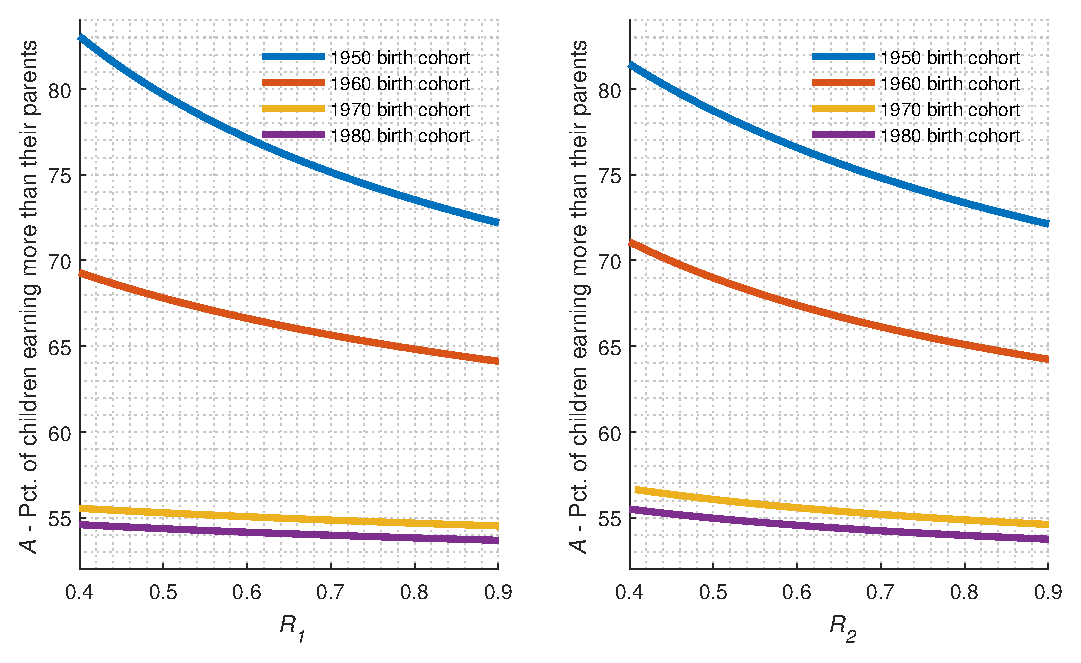
\includegraphics[width=1.0\textwidth] {./figs/R1_R2.eps}
\caption{The theoretical relationship between the rate of absolute mobility, $R_1$ (left) and $R_2$ (right), assuming the bivariate normal log-incomes model for different birth cohorts in the United States. This demonstrates the inverse relationship between absolute and relative mobility measures.}
\flabel{relat}
\end{figure}

\Pref{prop2} illustrates that the rate of absolute mobility increases with increasing income growth and decreases with increasing income inequality, as described by~\citet{chetty2017fading}. However, it also demonstrates that an additional mechanism can be at play, since the rate of absolute mobility decreases with increasing relative mobility. The direct implication is that if the relative mobility in the United States had been decreasing during the past few decades, as some argue~\citep{aaronson2008intergenerational,putnam2012growing}, the decrease in absolute mobility is less significant than reported by~\citet{chetty2017fading}.

\section{Discussion}

The counterintuitive inverse theoretical relationship found between absolute and relative mobility stems from a fundamental conceptual difference between the two categories of mobility. It exposes the problems that can arise if both are treated as measuring similarly the same phenomenon. In particular, absolute mobility is very sensitive to across-the-board economic growth. For example, during the Middle Ages -- when relative mobility rates were low because social class and profession were predominantly inherited~\citep{goldthorpe1982social,clark2014also}, even the slightest positive or negative income growth would result in very high or low absolute mobility. A misleading picture of intergenerational mobility may arise if the basic properties of these measures are overlooked. Therefore, empirically addressing this measure of intergenerational mobility requires careful delineation of the phenomena of interest and the manner in which quoted measures reflect them. In this study exposed this particular property of the absolute mobility measure.

From an empirical perspective, our findings imply that a model as simple as a bivariate log-normal distribution is satisfactory from describing the dynamics of absolute mobility. Thus, using available data on the marginal income distributions and on relative intergenerational mobility, one can produce estimates of absolute intergenerational mobility without the need for high-quality panel data sets, which remain unavailable in most countries.

\clearpage

\doublespacing
\bibliography{mobmob}

\clearpage

%\doublespacing

\appendix

\section{Proofs}
\label{app:appA}

\subsection{Proof of \preflong{prop1}}

First, by definition, the correlation $\rho$, between $X_p$ and $X_c$ equals to their covariance, divided by $\sigma_p\sigma_c$

\be
\rho = \frac{\text{Cov}\left[X_p,X_c\right]}{\sigma_p\sigma_c}\,.
\ee

$\beta$ can be directly calculated as follows, by the linear regression slope definition:

\be
\beta = \frac{\sum_{i=1}^{N} {\left(X_p^i - \bar{X}_p\right)\left(X_c^i - \bar{X}_c\right)}}{\sum_{i=1}^{N} {\left(X_p^i - \bar{X}_p\right)}}\,,
\ee
where $\bar{X}_p$ and $\bar{X}_c$ are the average parents and children log-incomes, respectively.

It follows that 
\be
\beta = \frac{\text{Cov}\left[X_p,X_c\right]}{\sigma_p^2}\,.
\ee

We immediately obtain

\be
\beta = \frac{\sigma_c}{\sigma_p}\rho
\ee

and therefore

\be
1-\beta = R_1 = 1-\frac{\sigma_c}{\sigma_p}\rho
\ee

\qed

\subsection{Proof of \preflong{prop2}}

We start by defining a new random variable $Z = X_c-X_p$. It follows that calculating $A$ is equivalent to calculating the probability $P\left(Z>0\right)$.

Subtracting two dependent normal distributions yields that

\be
Z \sim \mathcal{N}\left(\mu_c - \mu_p,\sigma_p^2 + \sigma_c^2 - 2\text{Cov}\left[X_p,X_c\right]\right)\,,
\ee

so according to \pref{prop1}

\be
Z \sim \mathcal{N}\left(\mu_c - \mu_p,\sigma_p^2\left(1-2\beta\right) + \sigma_c^2\right)\,.
\ee

If follows that

\be
\frac{Z - \left(\mu_c - \mu_p\right)}{\sqrt{\sigma_p^2\left(1-2\beta\right) + \sigma_c^2}} \sim \mathcal{N}\left(0,1\right)\,,
\ee

so we can now write

\be
\begin{split}
&P\left(Z>0\right) = \\ & P\left(\frac{Z - (\mu_c - \mu_p)}{\sqrt{\sigma_p^2\left(1-2\beta\right) + \sigma_c^2}} > -\frac{\mu_c - \mu_p}{\sqrt{\sigma_p^2\left(1-2\beta\right) + \sigma_c^2}} \right) = \\ &\Phi\left(\frac{\mu_c - \mu_p}{\sqrt{\sigma_p^2\left(1 - 2\beta\right) + \sigma_c^2}}\right) \,,
\end{split}
\ee
where $\Phi$ is the cumulative distribution function of the standard normal distribution.

\qed

\subsection{Proof of \creflong{coro1}}

For the bivariate log-normal model it is known that~\citep{trivedi2007copula}

\be
1-R_2 = \frac{6\arcsin{\frac{\rho}{2}}}{\pi}\,.
\ee

hence, using~\eref{beta_rho}

\be
R_2 = 1- \frac{6\arcsin{\frac{\sigma_p\beta}{2\sigma_c}}}{\pi}\,.
\ee

Substituting into~\eref{abs2} we obtain

\be
A = \Phi\left(\frac{\mu_c - \mu_p}{\sqrt{\sigma_p^2\left(1 - \frac{4\sigma_c}{\sigma_p}\sin{\left(\frac{\pi\left(1-R_2\right)}{6}\right)}\right) + \sigma_c^2}}\right) \,.
\ee

\qed

\section{Model robustness check}
\label{app:appB}

Our analysis was done for a bivariate log-normal model, assuming the marginal log-income distributions are normal and that their copula is Gaussian. This enables the derivation of \eref{abs2}, useful for investigating the relationship between absolute and relative mobility. This model for the joint income distributions of parents and children was found as unsatisfactory for some applications~\citep{bonhomme2009assessing}. Therefore, we wish to check how robust is this model when compared to other possible models.

For that purpose we assume two possible shapes for the marginal income distributions -- log-normal and gamma, both used in numerous studies as approximations of empirical income distributions~\citep{salem1974convenient,pinkovskiy2009parametric}. The historical parameters for the marginal distributions were calculated using data for the per capita pre-tax income in the United States~\citep{PikettyZucman2014} and the income share data~\citep{WID2017}, as described in~\ref{sec:results}.

In addition, we assume four possible copula forms -- Gaussian, Clayton, Gumbel and Plackett. Please refer to~\citet{trivedi2007copula} and~\citet{bonhomme2009assessing} for a discussion in uses of the different copula forms and their mathematical properties.

We test eight cases, assuming each form of copula assuming log-normal and gamma marginal distributions. For each case we use least squares fitting to fit one parameter, the copula dependence parameter $\theta$~\citep{trivedi2007copula}, so it best reproduces the measured $A$, reported by~\citet{chetty2017fading}. For each case we also calculate its root-mean-square deviation (RMSD) from the data and the relative absolute error (RAE).

The results of the robustness check are presented in~\tref{robust}. They show that using the gamma marginal distributions yields slightly higher $R^2$ than when using log-normal marginal distributions. However, using log-normal marginal distributions results in somewhat lower RMSD and RAE. None of the eight possible combinations of marginal distribution and copula stands out in particular.

\begin{table}[!htb]
\ra{1.1}
\centering
\captionof{table}{Model robustness check results}\tlabel{robust}
\begin{tabular}{@{}llccc@{}}\toprule[1.5pt]
Marginal distribution & Copula & $R^2$ & RMSD & RAE\\
\midrule[1.5pt]
\multirow{ 4}{*}{Log-normal}
& Gaussian & 0.767 & 0.051 & 0.355\\
& Clayton & 0.781 & 0.053 & 0.400\\
& Gumbel & 0.727 & 0.053 & 0.365\\
& Plackett & 0.750 & 0.052 & 0.364\\
\midrule[1.5pt]
\multirow{ 4}{*}{Gamma}
& Gaussian & 0.839 & 0.058 & 0.480\\
& Clayton & 0.712 & 0.080 & 0.602\\
& Gumbel & 0.839 & 0.050 & 0.385\\
& Plackett & 0.826 & 0.061 & 0.513\\
\bottomrule[1.5pt]
\end{tabular}
\end{table}

\Fref{copulas1} depicts the absolute intergenerational mobility resulting in each of the eight combinations in comparison to data. It shows that for the log-normal marginal distribution the differences between the different copulas is very small. The difference between the Gaussian and Plackett copulas is practically undetectable. This is also the case for the gamma marginal distribution. For the gamma marginal distribution, however, the calculated absolute intergenerational mobility shows a pronounced difference from the data for the birth cohorts of 1965--1980.

\begin{figure}[!htb]
\centering
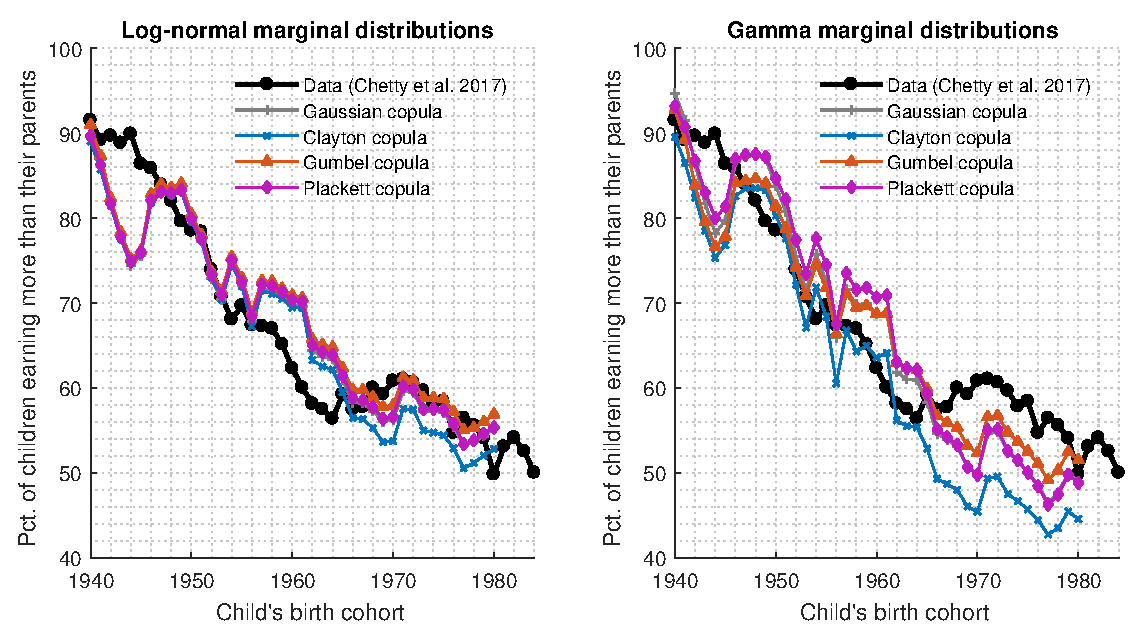
\includegraphics[width=1.0\textwidth]{./figs/copulas1.eps}
\caption{A comparison between the measured (black) and calculated absolute mobility for different copula forms. Left: using log-normal marginal distributions; Right: using gamma marginal distributions.}
\flabel{copulas1}
\end{figure}

The robustness check shows that the differences between the considered combinations are generally small. In particular, the Gaussian copula with log-normal marginal distributions provides results which are as good as the other combinations. Therefore, we conclude that for the purpose of modeling the dynamics of absolute mobility, the bivariate log-normal model is indeed a good model.

\end{document}